%%%%%%%%%%%%%%%%%%%%%%%%%%%%%%%%%%%%%%%%%%%
%
% From a template maintained at https://github.com/jamesrobertlloyd/cbl-tikz-poster
%
% Code near the top should be fairly standard and not need to be changed
%  - except for the document class
% Code lower down is more likely to be customised
%
%%%%%%%%%%%%%%%%%%%%%%%%%%%%%%%%%%%%%%%%%%%


\documentclass[landscape,a0b,final,a4resizeable]{include/a0poster}

\usepackage{multicol}
\usepackage{color}
\usepackage{morefloats}
\usepackage[pdftex]{graphicx}
\usepackage{rotating}
\usepackage{amsmath, amsthm, amssymb, bm}
\usepackage{array}
\usepackage{booktabs}
\usepackage{multirow}
\usepackage{hyperref}


\usepackage{include/picins}
\usepackage{tikz}
\usetikzlibrary{shapes.geometric,arrows,chains,matrix,positioning,scopes,calc}
\tikzstyle{mybox} = [draw=white, rectangle]
\definecolor{darkblue}{rgb}{0,0.08,0.45}
\definecolor{blue}{rgb}{0,0,1}

\usepackage{dsfont}

%%%%%%%%%%%%%%%%%%%%%%%%%%%%%%%%%%%%%%%%%%%
%
% myfig
%
% \myfig - replacement for \figure
% necessary, since in multicol-environment 
% \figure won't work        
%                 
%%%%%%%%%%%%%%%%%%%%%%%%%%%%%%%%%%%%%%%%%%%

\newcommand{\myfig}[3][0]{
\begin{center}
  \vspace{1.5cm}
  \includegraphics[width=#3\hsize,angle=#1]{#2}
  \nobreak\medskip
\end{center}}

%%%%%%%%%%%%%%%%%%%%%%%%%%%%%%%%%%%%%%%%%%%
%
% mycaption                
%
% \mycaption - replacement for \caption
% necessary, since in multicol-environment \figure and
% therefore \caption won't work
%
%%%%%%%%%%%%%%%%%%%%%%%%%%%%%%%%%%%%%%%%%%%

%\newcounter{figure}
\setcounter{figure}{1}
\newcommand{\mycaption}[1]{
  \vspace{0.5cm}
  \begin{quote}
    {{\sc Figure} \arabic{figure}: #1}
  \end{quote}
  \vspace{1cm}
  \stepcounter{figure}
}

%%%%%%%%%%%%%%%%%%%%%%%%%%%%%%%%%%%%%%%%%%%
%
% Some standard colours
%
%%%%%%%%%%%%%%%%%%%%%%%%%%%%%%%%%%%%%%%%%%%

\definecolor{camlightblue}{rgb}{0.601 , 0.8, 1}
\definecolor{camdarkblue}{rgb}{0, 0.203, 0.402}
\definecolor{camred}{rgb}{1, 0.203, 0}
\definecolor{camyellow}{rgb}{1, 0.8, 0}
\definecolor{lightblue}{rgb}{0, 0, 0.80}
\definecolor{white}{rgb}{1, 1, 1}
\definecolor{whiteblue}{rgb}{0.80, 0.80, 1}

%%%%%%%%%%%%%%%%%%%%%%%%%%%%%%%%%%%%%%%%%%%
%
% Some look and feel definitions
%
%%%%%%%%%%%%%%%%%%%%%%%%%%%%%%%%%%%%%%%%%%%

\setlength{\columnsep}{0.03\textwidth}
\setlength{\columnseprule}{0.0018\textwidth}
\setlength{\parindent}{0.0cm}

%%%%%%%%%%%%%%%%%%%%%%%%%%%%%%%%%%%%%%%%%%%
%
% \mysection - replacement for \section*
% 
% Puts a pretty box around some text
% TODO - any other thoughts for what this box should look like
%
%%%%%%%%%%%%%%%%%%%%%%%%%%%%%%%%%%%%%%%%%%%

\tikzstyle{mysection} = [rectangle, 
			draw=none, 
			shade, 
			outer color=camlightblue!00,
			inner color=camlightblue!00,
			text width=0.965\columnwidth,
			text centered,
			rounded corners=20pt,
			minimum height=0.09\columnwidth]

\newcommand{\mysection}[1]
{
\begin{center}
  \begin{tikzpicture}
    \node[mysection] {\sffamily\bfseries\huge#1};
  \end{tikzpicture}
\end{center}
}

%%%%%%%%%%%%%%%%%%%%%%%%%%%%%%%%%%%%%%%%%%%
%
% Set the font
%
% TODO - Not sure what a canonical choice is - feel free to modify
%
%%%%%%%%%%%%%%%%%%%%%%%%%%%%%%%%%%%%%%%%%%%

\renewcommand{\familydefault}{cmss}
\sffamily

%%%%%%%%%%%%%%%%%%%%%%%%%%%%%%%%%%%%%%%%%%%%%%%%%%%%
%%%               Background                     %%%
%%%%%%%%%%%%%%%%%%%%%%%%%%%%%%%%%%%%%%%%%%%%%%%%%%%%

\newcommand{\background}[3]{
  %\definecolor{cgradbegin}{#1}
  %\definecolor{cgradend}{#2}
 % \psframe[fillstyle=gradient,gradend=cgradend,
 % gradbegin=cgradbegin,gradmidpoint=#3](0.,0.)(1.\textwidth,-1.\textheight)
}




%%%%%%%%%%%%%%%%%%%%%%%%%%%%%%%%%%%%%%%%%%%%%%%%%%%%
%%%                pcolumn                       %%%
%%%%%%%%%%%%%%%%%%%%%%%%%%%%%%%%%%%%%%%%%%%%%%%%%%%%

\newenvironment{pcolumn}[1]{
  \begin{minipage}{#1\textwidth}
  \begin{center}
}{
  \end{center}
  \end{minipage}
}



%%%%%%%%%%%%%%%%%%%%%%%%%%%%%%%%%%%%%%%%%%%%%%%%%%%%
%%%                pbox                          %%%
%%%%%%%%%%%%%%%%%%%%%%%%%%%%%%%%%%%%%%%%%%%%%%%%%%%%

\definecolor{lcolor}{rgb}{0, 0, 0.80}
\definecolor{gcolor1}{rgb}{1, 1, 1}
\definecolor{gcolor2}{rgb}{.80, .80, 1}

  % \def\fc{fillcolor}
  % \def\getfc #1=#2\par{\def\ffc{#1} \ifx\ffc\fc #2\fi} 
  % \def\getfillcolor #1,#2\par{\getfc #1\par \getfc #2\par}

 %  \newcommand{\psshadowbox}[2]{%[2][magenta]{
%      \fbox{Input arg: #1}
%      \fbox{#1} 
%      \fbox {\getfillcolor #1\par}
%      \def\col{\getfillcolor #1\par}
 
%      \let\coll=\col
%       \coll
 %     \colorbox{\col}{#2}
%       \mbox
   %   \coloredshadowbox{black}{\coll}{#2}
%   }

\newcommand{\pbox}[4]{
%\psshadowbox[#3]{
%\fbox{
\mbox{
\begin{minipage}[t][#2][t]{#1}
#4
\end{minipage}
}%}
}

%%%%%%%%%%%%%%%%%%%%%%%%%%%%%%%%%%%%%%%%%%%
%
% Poster environment
%
% Centres everything and can be used to define the width of the content
%
%%%%%%%%%%%%%%%%%%%%%%%%%%%%%%%%%%%%%%%%%%%

\newenvironment{poster}{
  \begin{center}
  \begin{minipage}[c]{\textwidth}
}{
  \end{minipage}
  \end{center}
}

\def\newarrow{\mbox{\begin{tikzpicture}
             \useasboundingbox{(-3pt,-4.5pt) rectangle (19pt,1pt)};
             \draw[->] (0,-0.07)--(17pt,-0.07);\end{tikzpicture}}}



\ProvidesPackage{preamble}

\usepackage{url}
\usepackage{array}
\usepackage{amsmath,amssymb,amsfonts,textcomp}
\usepackage{booktabs}
\usepackage{relsize}
\usepackage{nicefrac}
\usepackage{graphicx}
\usepackage{rotating}
\usepackage{nth}
\usepackage{acronym}
\usepackage{bm}

\newcommand{\binarysum}{\sum_{\bf{x} \in \{0,1\}^D}}
\newcommand{\expect}{\mathbb{E}}
\newcommand{\expectargs}[2]{\mathbb{E}_{#1} \left[ {#2} \right]}
\newcommand{\var}{\mathbb{V}}
\newcommand{\varianceargs}[2]{\mathbb{V}_{#1} \left[ {#2} \right]}
\newcommand{\variance}{\mathbb{V}}
\newcommand{\cov}{\operatorname{cov}}
\newcommand{\Cov}{\operatorname{Cov}}
\newcommand{\covarianceargs}[2]{\Cov_{#1} \left[ {#2} \right]}
\newcommand{\colvec}[2]{\left[ \begin{array}{c} {#1} \\ {#2} \end{array} \right]}
\newcommand{\tbtmat}[4]{\left[ \begin{array}{cc} {#1} & {#2} \\ {#3} & {#4} \end{array} \right]}

%\newcommand{\covskinny}[2]{\var\!\left(#1\middle\vert#2\right)} 

\newcommand{\acro}[1]{\textsc{#1}}
%\newcommand{\vect}[1]{\boldsymbol{#1}}
\newcommand{\vect}[1]{{\bf{#1}}}
\newcommand{\mat}[1]{\mathbf{#1}}
\newcommand{\pderiv}[2]{\frac{\partial #1}{\partial #2}}
\newcommand{\npderiv}[2]{\nicefrac{\partial #1}{\partial #2}}

\newcommand{\pha}{^{\phantom{:}}}

\newcommand{\argmin}{\operatornamewithlimits{argmin}}
\newcommand{\argmax}{\operatornamewithlimits{argmax}}

% The following designed for probabilities with long arguments

\newcommand{\Prob}[2]{P\!\left(\,#1\;\middle\vert\;#2\,\right)}
\newcommand{\ProbF}[3]{P\!\left(\,#1\!=\!#2\;\middle\vert\;#3\,\right)}
\newcommand{\p}[2]{p\!\left(#1\middle\vert#2\right)}
\newcommand{\po}[1]{p\!\left(#1\right)}
\newcommand{\pF}[3]{p\!\left(\,#1\!=\!#2\;\middle\vert\;#3\,\right)} 
\newcommand{\mean}[2]{{m}\!\left(#1\middle\vert#2\right)}
%\newcommand{\novmean}[2]{{m}\!\left(#1\middle\vert#2\right)}
%\newcommand{\novcov}[2]{\var\!\left(#1\middle\vert#2\right)}
%\newcommand{\cov}[2]{\var\!\left(#1\middle\vert#2\right)} 
%\newcommand{\pskinny}[2]{p\!\left(#1\;\middle\vert\;#2\right)}
%\newcommand{\meanskinny}[2]{{m}\!\left(#1\middle\vert#2\right)}
%\newcommand{\covskinny}[2]{\var\!\left(#1\middle\vert#2\right)} 

\newcommand{\vI}{\mat{I}}
\newcommand{\vX}{\mat{X}}
\newcommand{\vY}{\mat{Y}}
\newcommand{\vZ}{\mat{Z}}
\newcommand{\vK}{\mat{K}}
\newcommand{\vi}{\vect{i}}
\newcommand{\vs}{\vect{s}}
\newcommand{\va}{\vect{a}}
\newcommand{\vA}{\vect{A}}
\newcommand{\vb}{\vect{b}}
\newcommand{\vB}{\mat{B}}
\newcommand{\vr}{\mat{r}}
\newcommand{\vR}{\mat{R}}
\newcommand{\vS}{\mat{S}}
\newcommand{\vu}{\vect{u}}
\newcommand{\vv}{\vect{v}}
\newcommand{\vk}{\vect{k}}
\newcommand{\vc}{\vect{c}}
\newcommand{\vC}{\mat{C}}
\newcommand{\vw}{\vect{w}}
\newcommand{\vx}{\vect{x}}
\newcommand{\vy}{\vect{y}}
\newcommand{\vz}{\vect{z}}
\newcommand{\vmu}{\vect{\mu}}
\newcommand{\vpi}{\vect{\pi}}
\newcommand{\vphi}{\vect{\phi}}
\newcommand{\vSigma}{\mat{\Sigma}}
\newcommand{\vtheta}{\vect{\theta}}
\newcommand{\vl}{\vect{l}}
\newcommand{\vq}{\vect{q}}
\newcommand{\vf}{\vect{f}}
\newcommand{\vg}{\vect{g}}
\newcommand{\vell}{\vect{\ell}}
\newcommand{\ve}{\vect{\epsilon}}
\newcommand{\vzero}{\vect{0}}
\newcommand{\vone}{\vect{1}}

\newcommand{\He}{\mathcal{H}}
\newcommand{\normx}[2]{\left\|#1\right\|_{#2}}
\newcommand{\Hnorm}[1]{\normx{#1}{\He}}
\newcommand{\mmd}{{\rm MMD}}


\newcommand{\mf}{\bar{\vf}}

\newcommand{\st}{_\star}

\newcommand{\inv}{^{{\mathsmaller{-1}}}}
\newcommand{\tohalf}{^{{\mathsmaller{\nicefrac{1}{2}}}}}

\newcommand{\N}[3]{\mathcal{N}\!\left(#1|#2,#3\right)}
\newcommand{\bN}[3]{\mathcal{N}\big(#1|#2,#3\big)}
\newcommand{\boldN}[3]{\text{\textbf{\mathcal{N}}}\big(#1;#2,#3\big)}
\newcommand{\ones}[1]{\mat{1}_{#1}}
\newcommand{\eye}[1]{\mat{E}_{#1}}
\newcommand{\tra}{^\ensuremath{\mathsf{T}}}
\newcommand{\trace}{\operatorname{tr}}
\newcommand{\deq}{:=}
\newcommand{\degree}{^\circ}

\DeclareMathOperator{\chol}{chol}
\DeclareMathOperator{\diag}{diag}

\newcommand{\gp}{{\acro{gp}}}
\newcommand{\bmc}{{\acro{bmc}}}
\newcommand{\bq}{{\acro{bq}}}
\newcommand{\sbq}{{\acro{sbq}}}

\newenvironment{narrow}[2]{%
  \begin{list}{}{%
  \setlength{\topsep}{0pt}%
  \setlength{\leftmargin}{#1}%
  \setlength{\rightmargin}{#2}%
  \setlength{\listparindent}{\parindent}%
  \setlength{\itemindent}{\parindent}%
  \setlength{\parsep}{\parskip}}%
\item[]}{\end{list}}

\newtheorem{prop}{Proposition}
\newtheorem{cor}{Corollary}
\newtheorem{lem}{Lemma}


\def\ie{i.e.\ }
\def\eg{e.g.\ }
\def\iid{i.i.d.\ }
\def\simiid{\sim_{\mbox{\tiny iid}}}
\def\eqdist{\stackrel{\mbox{\tiny d}}{=}}

\def\Reals{\mathbb{R}}

\def\Uniform{\mbox{\rm Uniform}}
\def\Bernoulli{\mbox{\rm Bernoulli}}
\def\GP{\mathcal{GP}}

\def\inputVar{x}
\def\InputVar{X}
\def\InputSpace{\mathcal{X}}
\def\outputVar{y}
\def\OutputSpace{\mathcal{Y}}
\def\function{f}
\def\kernel{k}
\def\KernelMatrix{K}
\def\SumKernel{\sum}
\def\ProductKernel{\prod}
\def\expression{e}

\def\SE{\acro{SE}}
\def\Per{\acro{Per}}
\def\RQ{\acro{RQ}}
\def\Lin{\acro{Lin}}

\def\subexpr{{\cal S}}
\def\baseker{{\cal B}}
\def\numWinners{k}

\newcommand{\kSE}{{\acro{SE}}}
\newcommand{\kC}{{\acro{C}}}
\newcommand{\kPer}{{\acro{Per}}}
\newcommand{\kLin}{{\acro{Lin}}}
\newcommand{\kWN}{{\acro{WN}}}
\newcommand{\kCP}{{\acro{CP}}}
\newcommand{\kCW}{{\acro{CW}}}
\newcommand{\kRQ}{{\acro{RQ}}}

\newcommand{\vv}{\mathbf{v}}

\begin{document}
\begin{poster} 

% Potentially add some space at the top of the poster
\vspace{0\baselineskip}


%%% Header
\begin{center}
\begin{pcolumn}{0.99}

\newcommand{\logowidth}{0.099\textwidth}

\pbox{0.99\textwidth}{}{linewidth=2mm,framearc=0.3,linecolor=camdarkblue,fillstyle=gradient,gradangle=0,gradbegin=white,gradend=white,gradmidpoint=1.0,framesep=1em}{
%
%%% Cambridge Logo
\begin{minipage}[c]{\logowidth}
  \begin{center}
    \includegraphics[width=18cm]{badges/hips-logo.png}
  \end{center}
\end{minipage}
%
%%% Title
\begin{minipage}[c][9cm][c]{0.76\textwidth}
  \begin{center}
    {\sffamily \VeryHuge \textbf{Convolutional Networks on Graphs \\for Learning Molecular Fingerprints}}\\[10mm]
    {\huge\sffamily \Huge David Duvenaud*, Dougal Maclaurin*, Jorge Aguilera-Iparraguirre \\ Rafael G\'omez-Bombarelli, Timothy Hirzel, Al\'an Aspuru-Guzik, Ryan P. Adams\\[7.5mm]
    %\texttt{\{ti242, dkd23, zoubin\}@cam.ac.uk}
    }
  \end{center}
\end{minipage}
%
%
% Harvard logo
\begin{minipage}[c]{\logowidth}
  \begin{flushright}
    \includegraphics[width=8cm,trim=2em 0em 2em 2em, clip]{badges/harvard}
  \end{flushright}
\end{minipage}
%
}
\end{pcolumn}
\end{center}

\vspace*{1.5cm}

\Large


%%%%%%%%%%%%%%%%%%%%%%%%%%%%%%%%%%%%%%%%%%%%%%%%%%%%%%%%%%%%%%%%%%%%%%
%%% Beginning of Document
%%%%%%%%%%%%%%%%%%%%%%%%%%%%%%%%%%%%%%%%%%%%%%%%%%%%%%%%%%%%%%%%%%%%%%


\begin{multicols}{3}

\mysection{Problem}

\vspace{-0.5in}

\begin{tabular}{cc}
\begin{minipage}[c]{0.5\columnwidth}
\begin{itemize}
  \item How to do regression when input is a graph?
  \item Graphs can be any size or shape.
  \item Hard to turn into fixed-length vector.
  \item Molecules are graphs!
  \item Australians are \emph{it}
\end{itemize}
\end{minipage} & 
\begin{minipage}[c]{0.5\columnwidth}
%\includegraphics[width=\columnwidth]{../talks/talkfigs/learning_curves_3.pdf}
\centerline{\includegraphics[width=1.0\columnwidth, clip, trim=4mm 10mm 4mm 4mm]{figures/how-fingerprints.png}}
\end{minipage}
\end{tabular}

\vspace{-0.5in}

\mysection{Circular fingerprints}

Aka Morgan fingerprints, or ECFP

\begin{tabular}{cc}
\begin{minipage}[c]{0.5\columnwidth}
\begin{itemize}
  \item Map variable-sized molecular graph to fixed-length binary vector
  %\item Does this by hashing self with neighbors iteratively
  \item Binary features indicate presence of substructures
\end{itemize}

Can be efficiently computed using local operations:

\begin{itemize}
  \item At each layer, hash the features of each atom and its neighbors/bonds
  \item More layers correspond to increasing radius of substructures
  \item At top level, interpret as (modulo) integer and set the entry to one
\end{itemize}
\end{minipage} & 
\begin{minipage}[c]{0.5\columnwidth}
%\includegraphics[width=\columnwidth]{../talks/talkfigs/learning_curves_3.pdf}
\centerline{\includegraphics[width=0.9\columnwidth, clip, trim=4mm 12mm 4mm 4mm]{figures/fig_1}}
\end{minipage}
\end{tabular}



\newpage %%%%%%%%%%%%%%%%%%%%%%%%%%%%%%%%%%%%%%%%%%%%%%%%%%%%%%%%%%%%%%%%%%%%%%%%%%%%%%%%%%%%%%%%%%%%%%%


\mysection{Convolutional neural nets on graphs}

\vspace{0.5in}

\begin{tabular}{cc}
\begin{minipage}[c]{0.5\columnwidth}

How to make these differentiable?

\begin{center}
\begin{tabular}{rcl}
Hash  & $\rightarrow$ & neural net \\
Index & $\rightarrow$ & softmax \\
Write & $\rightarrow$ & Add
\end{tabular}
\end{center}

Results in an end-to-end differentiable convolutional network

\end{minipage} & 
\begin{minipage}[c]{0.4\columnwidth}
\begin{center}
Information flow graph

\hspace{-1em}\centerline{\includegraphics[width=\columnwidth, clip, trim=4mm 12mm 4mm 4mm]{figures/3d-nets/net1.png}}
\end{center}

Message passing between neighbors, plus final pooling step

\end{minipage}
\end{tabular}

\vspace{0.5in}

\mysection{Neural fingerprints are interpretable}

\newcommand{\mywidtha}{8cm}
\newcommand{\mywidthb}{10cm}

When trained with linear layer on top, can see which fragments most contribute to prediction.

\begin{center}
%\newcommand{\molfeature}[3]{\includegraphics[width=#3, clip, trim = 2mm 3mm 2mm 6mm]{fig_4.pdf}\vspace{-1em}}%
%\begin{figure}[h]%
\vspace{-1em}
\begin{tabular}{>{\centering}m{\mywidthb} >{\centering}m{\mywidtha} >{\centering}m{\mywidtha} >{\centering\arraybackslash}m{\mywidtha}}
Fragments most activated by pro-solubility feature & 
%\molfeature{15}{0}{3.3cm} & \molfeature{15}{3}{3.3cm} & \molfeature{15}{2}{2.5cm}\\
\includegraphics[width=\mywidtha, clip, trim = 2mm 3mm 2mm 6mm]{figures/fig_5.pdf}\vspace{-1em} &
\includegraphics[width=\mywidtha, clip, trim = 2mm 3mm 2mm 6mm]{figures/fig_6.pdf}\vspace{-1em} &
\includegraphics[width=\mywidtha, clip, trim = 2mm 3mm 2mm 6mm]{figures/fig_7.pdf}\vspace{-1em} \\
\midrule
Fragments most activated by anti-solubility feature & 
%\molfeature{18}{4}{3.3cm} & \molfeature{18}{1}{3.3cm} & \molfeature{18}{2}{3.3cm}
\includegraphics[width=\mywidtha, clip, trim = 2mm 3mm 2mm 6mm]{figures/fig_8.pdf}\vspace{-1em} &
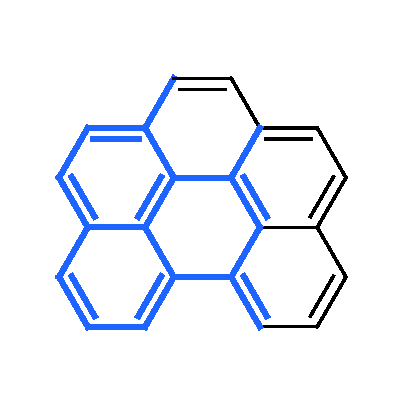
\includegraphics[width=\mywidtha, clip, trim = 2mm 3mm 2mm 6mm]{figures/fig_9.pdf}\vspace{-1em} &
\includegraphics[width=\mywidtha, clip, trim = 2mm 3mm 2mm 6mm]{figures/fig_10.pdf}\vspace{-1em} \\
%\end{tabular}
%\end{center}
\midrule
%\subsection{Toxicity features}
%We trained the same model architecture to predict toxicity in two different datasets.
%Shows fragments which maximally activate the feature most predictive of toxicity, in two separate datasets.
%\newcommand{\molfeaturetox}[2]{\includegraphics[width=3.4cm, clip, trim = 1mm 3mm 1mm 3mm]{fig_11.pdf}}%
%\begin{figure}[h]
%\begin{center}
%\begin{tabular}{>{\centering}m{\mywidthb} >{\centering}m{\mywidtha} >{\centering}m{\mywidtha} >{\centering\arraybackslash}m{\mywidtha}}
Fragments most activated by toxicity feature on SR-MMP dataset
& \includegraphics[width=\mywidtha]{figures/jorge-figures/7.png} 
& \includegraphics[width=\mywidtha]{figures/jorge-figures/8.png}
& \includegraphics[width=\mywidtha]{figures/jorge-figures/9.png}\\
\midrule
Fragments most activated by toxicity feature on NR-AHR dataset
%& \molfeaturetox{7}{14} & \molfeaturetox{7}{6} & \molfeaturetox{7}{5}
& \includegraphics[width=\mywidtha]{figures/jorge-figures/10.png} 
& \includegraphics[width=\mywidtha]{figures/jorge-figures/11.png}
& \includegraphics[width=\mywidtha]{figures/jorge-figures/12.png}\\
\end{tabular}
\vspace{-3mm}
%\caption{
\end{center}

%Visualizing fingerprints optimized for predicting toxicity.
%Shown here are representative samples of molecular fragments (highlighted in red) which most activate the feature most predictive of toxicity.

%\emph{Top row:} the most predictive feature identifies groups containing a sulphur atom attached to an aromatic ring.
%\emph{Bottom row:} the most predictive feature identifies fused aromatic rings, also known as polycyclic aromatic hydrocarbons, a well-known carcinogen.




\newpage %%%%%%%%%%%%%%%%%%%%%%%%%%%%%%%%%%%%%%%%%%%%%%%%%%%%%%%%%%%%%%%%%%%%%%%%%%%%%%%%%%%%%%%%%%%%%%%


\mysection{Neural graph fingerprints generalize circular fingerprints}

With large random weights, neural graph fingerprints approach circular fingeprints:

\begin{tabular}{cc}
\begin{minipage}[c]{0.45\columnwidth}
\includegraphics[width=\columnwidth]{figures/fig_2.pdf}
\end{minipage} & 
\begin{minipage}[c]{0.45\columnwidth}
\begin{center}
\vspace{0.5cm}\includegraphics[width=\columnwidth]{figures/fig_3.pdf}
\end{center}
\end{minipage}
\end{tabular}

\vspace{0.5em}

\mysection{Results}

Because neural graph fingerprints generalize state of the art, we can't not win:

\begin{center}
\begin{tabular}{r|lll}
Dataset                      &   Solubility  & Drug efficacy & Photovoltaic efficiency \\
\midrule
Units                        &   log Mol/L                            & EC$_{50}$ in nM                        & percent \\
\midrule
Predict mean                 & 2.07 $\pm$ 0.10        & 1.21 $\pm$ 0.03         & 2.53 $\pm$ 0.02 \\
Circular FPs + linear layer  & 1.31 $\pm$ 0.05        & \bf{1.06} $\pm$ 0.01    & 1.62 $\pm$ 0.03 \\
Circular FPs + neural net    & 1.18 $\pm$ 0.05        & 1.16 $\pm$ 0.04         & 1.41 $\pm$ 0.03 \\ 
Neural FPs + linear layer    & 0.87 $\pm$ 0.06        & \bf{1.07} $\pm$ 0.01    & 1.61 $\pm$ 0.06 \\  
Neural FPs + neural net      & \bf{0.72} $\pm$ 0.05   & \bf{1.08} $\pm$ 0.01    & \bf{1.20} $\pm$ 0.04
\end{tabular}

Mean predictive accuracy of neural fingerprints compared to standard circular fingerprints.
\end{center}


\vspace{0.5em}

\mysection{Conclusion}

\begin{itemize}
\item We can compute gradients of learning procedures...
\item This lets us optimize thousands of hyperparameters!
\item All code for experiments at \url{github.com/HIPS/hypergrad}
\item We also wrote an autodiff package that works on standard Numpy code:\\ \url{github.com/HIPS/autograd}
\end{itemize}



\end{multicols}
\end{poster}

\end{document}

